%* 
%* ------------------------------------------------------------------
%* DispatcherExamples.tex - Dispatcher Examples
%* Created by Robert Heller on Sat Jun 14 10:03:06 2008
%* ------------------------------------------------------------------
%* Modification History: $Log$
%* Modification History: Revision 1.1  2002/07/28 14:03:50  heller
%* Modification History: Add it copyright notice headers
%* Modification History:
%* ------------------------------------------------------------------
%* Contents:
%* ------------------------------------------------------------------
%*  
%*     Model RR System, Version 2
%*     Copyright (C) 1994,1995,2002-2005  Robert Heller D/B/A Deepwoods Software
%* 			51 Locke Hill Road
%* 			Wendell, MA 01379-9728
%* 
%*     This program is free software; you can redistribute it and/or modify
%*     it under the terms of the GNU General Public License as published by
%*     the Free Software Foundation; either version 2 of the License, or
%*     (at your option) any later version.
%* 
%*     This program is distributed in the hope that it will be useful,
%*     but WITHOUT ANY WARRANTY; without even the implied warranty of
%*     MERCHANTABILITY or FITNESS FOR A PARTICULAR PURPOSE.  See the
%*     GNU General Public License for more details.
%* 
%*     You should have received a copy of the GNU General Public License
%*     along with this program; if not, write to the Free Software
%*     Foundation, Inc., 675 Mass Ave, Cambridge, MA 02139, USA.
%* 
%*  
%* 

\chapter{Dispatcher Examples}
\label{chpt:dispatcher:Examples}
\typeout{$Id$}

These are four examples created using the Dispatcher program.  The code
files are included and can be used as references or even modified to
suit some part of your layout.

\section{Example 1: Simple siding on single track mainline}

\begin{figure}[hbpt]
\begin{centering}
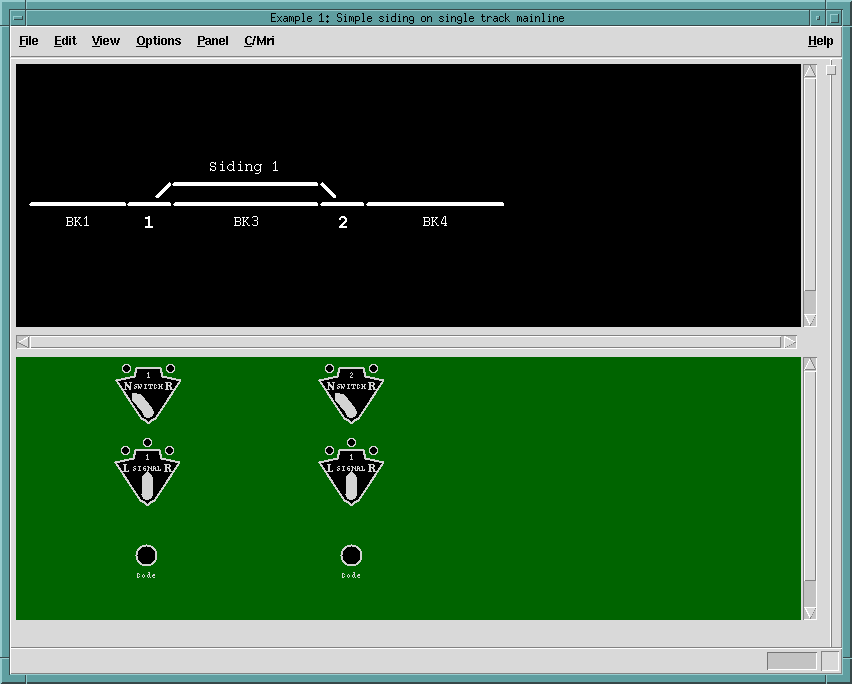
\includegraphics[width=5in]{DISPExample1.png}
\caption{Example 1: Simple siding on single track mainline}
\label{fig:dispatcher:example1}
\end{centering}
\end{figure}
\lstinputlisting[caption={Example 1: Simple siding on single track mainline},
		 label={lst:dispatcher:example1},
		 firstline=343]{example1.tcl}
\lstinputlisting[caption={Example 1: I/O Worksheet},
		 label={lst:dispatcher:example1wsh},
		 firstline=37]{example1.iow}
This example, shown in Figure~\ref{fig:dispatcher:example1}, with user
code in Listing~\ref{lst:dispatcher:example1} implements a simple
passing siding on a single track main line.  There are two control
points, one at each end of the siding.  Both control points are handled
with a single SMINI board.

\section{Example 2: Mainline with an industrial siding}

\begin{figure}[hbpt]
\begin{centering}
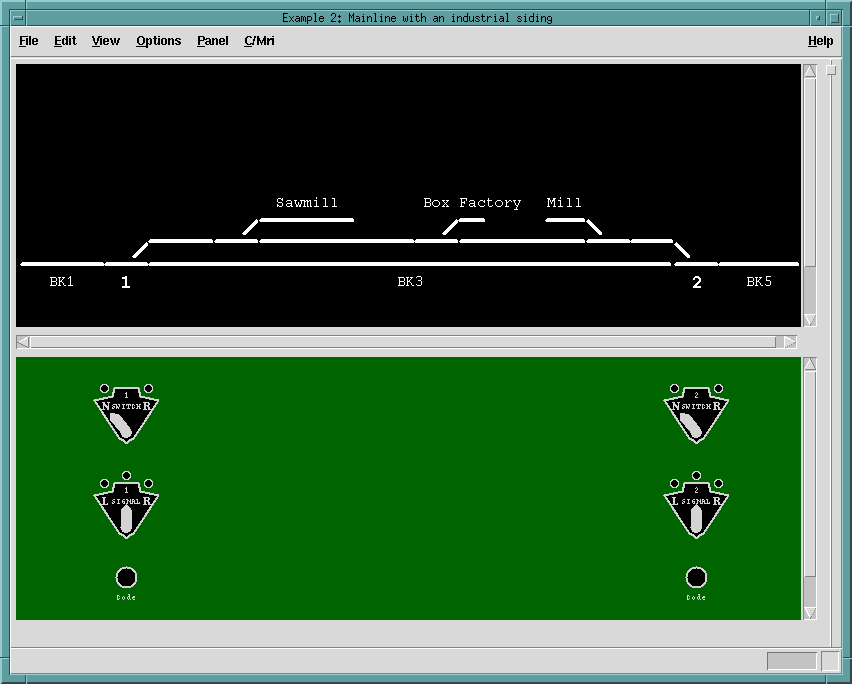
\includegraphics[width=5in]{DISPExample2.png}
\caption{Example 2: Mainline with an industrial siding}
\label{fig:dispatcher:example2}
\end{centering}
\end{figure}
\lstinputlisting[caption={Example 2: Mainline with an industrial siding},
		 label={lst:dispatcher:example2},
		 firstline=417]{example2.tcl}
\lstinputlisting[caption={Example 2: I/O Worksheet},
		 label={lst:dispatcher:example2wsh},
		 firstline=37]{example2.iow}
This example, shown in Figure~\ref{fig:dispatcher:example2}, with user
code in Listing~\ref{lst:dispatcher:example2} implements an industrial
siding on a single track main line.  There are two control points, one
at each end of the siding.  This example uses three SMINI boards, one
for each control point and one for the siding.

\section{Example 3: double track crossover}

\begin{figure}[hbpt]
\begin{centering}
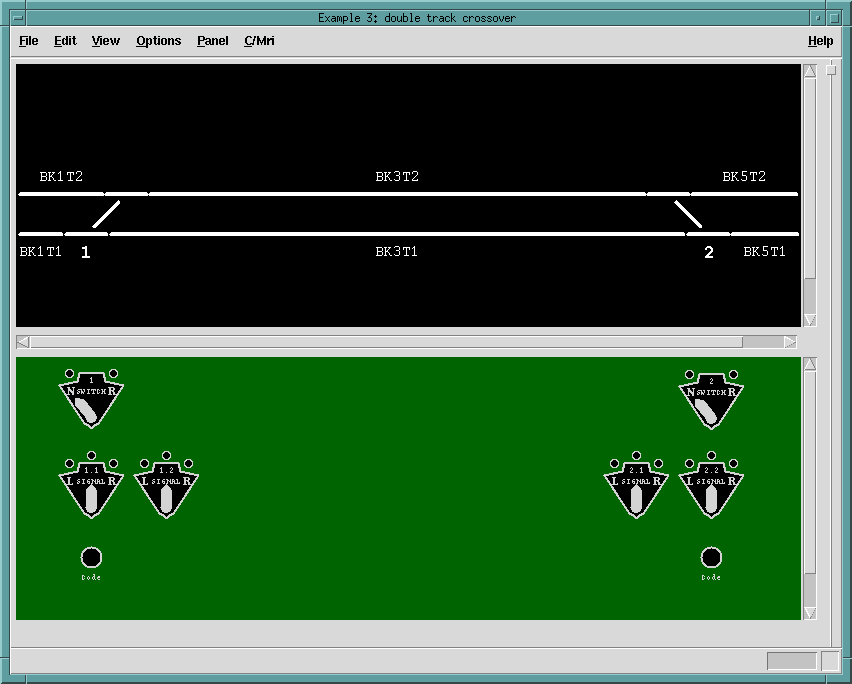
\includegraphics[width=5in]{DISPExample3.png}
\caption{Example 3: Double track crossover}
\label{fig:dispatcher:example3}
\end{centering}
\end{figure}
\lstinputlisting[caption={Example 3: Double track crossover},
		 label={lst:dispatcher:example3},
		 firstline=388]{example3.tcl}
\lstinputlisting[caption={Example 3: I/O Worksheet},
		 label={lst:dispatcher:example3wsh},
		 firstline=37]{example3.iow}
This example, shown in Figure~\ref{fig:dispatcher:example3}, with user
code in Listing~\ref{lst:dispatcher:example3} implements a double track
crossover. Uses two SMINI boards, one for each of the two control points.

\section{Example 4: From Chapter 9 of C/MRI User's Manual V3.0}

\begin{figure}[hbpt]
\begin{centering}
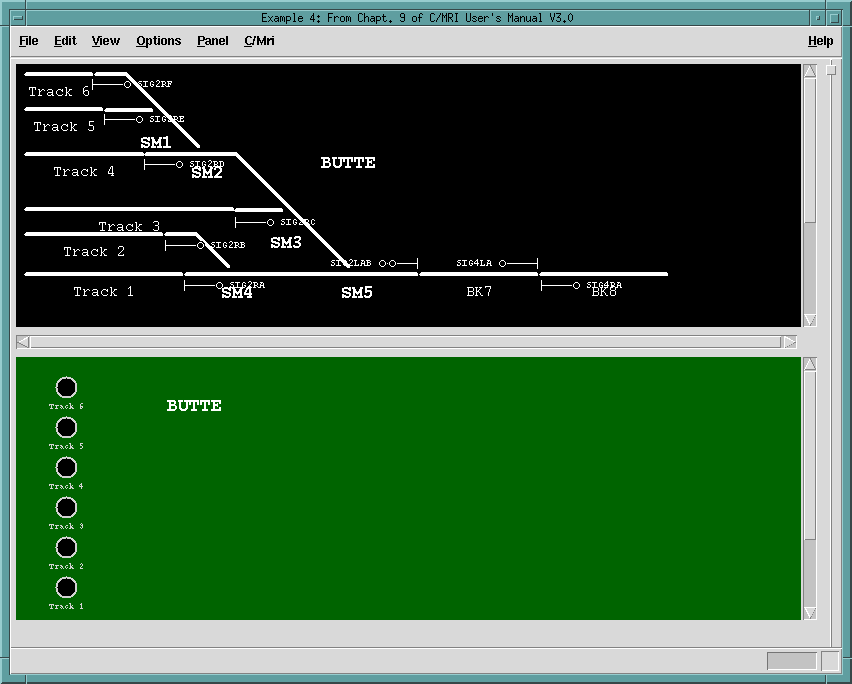
\includegraphics[width=5in]{DISPExample4.png}
\caption{Example 3: From Chapter 9 of C/MRI User's Manual V3.0}
\label{fig:dispatcher:example4}
\end{centering}
\end{figure}
\lstinputlisting[caption={Example 4: From Chapter 9 of C/MRI User's 
Manual V3.0},
		 label={lst:dispatcher:example4},
		 firstline=605]{example4.tcl}
\lstinputlisting[caption={Example 4: I/O Worksheet},
		 label={lst:dispatcher:example4wsh},
		 firstline=1]{example4.iow}
This example, shown in Figure~\ref{fig:dispatcher:example4}, with user
code in Listing~\ref{lst:dispatcher:example4} implements the yard
example from Chapter 9 of C/MRI User's Manual V3.0\cite{Chubb03}.  This
example uses a single SMINI board.  The physical push buttons are
replaced by ``virtual'' push buttons on the computer screen.  Otherwise,
this code is a drop-in replacement, in Tcl under Linux, for the Quick
BASIC code under MS-Windows included in Bruce Chubb's manual.

